% Native-TeX homotopy diagrams from LNM 239, physical p.21 / printed p.3.
\newcommand{\IllusieHomotopyTriangle}{%
  \begin{center}
  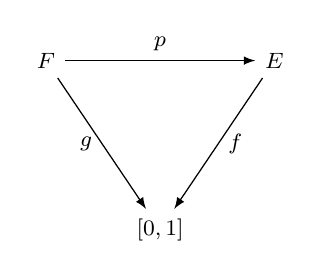
\begin{tikzpicture}[
    >=latex,
    line width=0.45pt,
    every node/.style={font=\rmfamily\fontsize{8}{9}\selectfont}
  ]
    \node (F) at (-1.45,1.0) {$F$};
    \node (E) at (1.45,1.0) {$E$};
    \node (I) at (0,-1.15) {$[0,1]$};
    \draw[->] (F) -- node[above] {$p$} (E);
    \draw[->] (F) -- node[left] {$g$} (I);
    \draw[->] (E) -- node[right] {$f$} (I);
  \end{tikzpicture}
  \end{center}%
}

\newcommand{\IllusieHomotopySquare}{%
  \begin{center}
  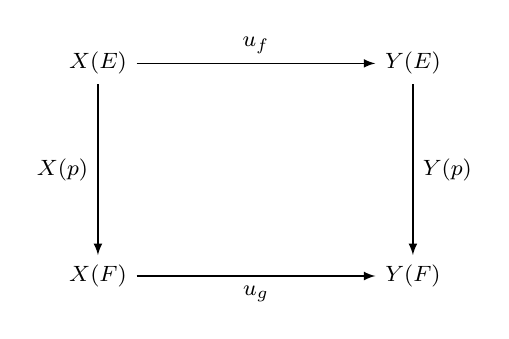
\begin{tikzpicture}[
    >=latex,
    line width=0.45pt,
    every node/.style={font=\rmfamily\fontsize{8}{9}\selectfont}
  ]
    \node (XE) at (-2.0,1.35) {$X(E)$};
    \node (YE) at (2.0,1.35) {$Y(E)$};
    \node (XF) at (-2.0,-1.35) {$X(F)$};
    \node (YF) at (2.0,-1.35) {$Y(F)$};
    \draw[->] (XE) -- node[above] {$u_f$} (YE);
    \draw[->] (XE) -- node[left] {$X(p)$} (XF);
    \draw[->] (YE) -- node[right] {$Y(p)$} (YF);
    \draw[->] (XF) -- node[below] {$u_g$} (YF);
  \end{tikzpicture}
  \end{center}%
}
